\chapter{国内外相关研究现状}\label{chap:related_work}

目前,国内外针对从非结构化文本中进行需求发现和提取已经有一些论文成果。在许多开源和工业项目中,开发人员大量使用书面沟通渠道,例如邮件列表,issue tracker、聊天工具等,并且这样的方式已经遍布全球开发人员的日产工作中。本文主要从@@@@@@几方面介绍国内外相关研究工作。

\section{基于文本数据的需求发现}

\subsection{基于规则的需求发现}

邮件是开发者之间进行沟通的重要方式之一,通常包含特征请求、观点询问、问题发现、解决方案、信息提供等不同类别的信息。Andrea Di Sorbo \cite{Sorbo2016Development}等人提出一种名叫DECA(开发者电子邮件内容分析器)的半监督学习方法,通过使用自然语言解析工具分析文本的语言学特征并且从询问帮助、提供帮助、提出新需求、报告或者讨论BUG等几方面对开发者的意图进行分类。Sorbo等人首先根据来自Ubuntu和QT的数据设置更适合邮件列表信息的分类,具体分类类别如表\ref{tab:deca0}所示:

\begin{table}[htbp]
\bicaption{这是一个样表。}{This is a sample table.}
    \label{tab:deca0}
    \centering
    \footnotesize% fontsize
    \setlength{\tabcolsep}{4pt}% column separation
    \renewcommand{\arraystretch}{1.2}%row space 
\begin{tabular}{lcccccccc}
\hline
句子类别的例子      & 分类类别 \\
\hline
讨论一个变更       & 特征请求 \\
定位BUG        & 问题发现 \\
BUG是否被修复     & 信息询问 \\
针对已知问题提出解决方案 & 解决方案 \\
请求其他开发者做出变更  & 特征请求 \\
询问代码时如何工作的   & 信息询问 \\
询问为何这样写代码    & 信息询问 \\
向某人征求意见      & 意见询问 \\
找出代码作者       & 信息询问 \\
更多的了解代码      & 信息询问 \\
告诉其他开发者一些事情  & 信息提供 \\
\hline
\end{tabular}
\end{table}


然后对其进行手工标注,作者发现开发人员在关于开发问题的讨论中撰写关于现有错误或者建议提出特征请求时,他们倾向于使用一些经常性的语言模式,比如对于“我们可以使用漏桶算法来限制带宽”,可以发现句子中提供一个明确定义的谓词-参数结构,对此,可以看出大多数具有谓词-论元结构的句子表明解决方案。作者定义了启发式规则,首先发现句子的特定句法结构,然后推广某些类型的信息,最后忽略无用的信息。所以,作者定义了“【某人】可以使用【某事物】”的一般模式来识别解决方案。图\ref{fig:deca1}是作者通过斯坦福依存句法分析来分析启发式规则时的例子:

\begin{figure}[!htbp]
    \centering
    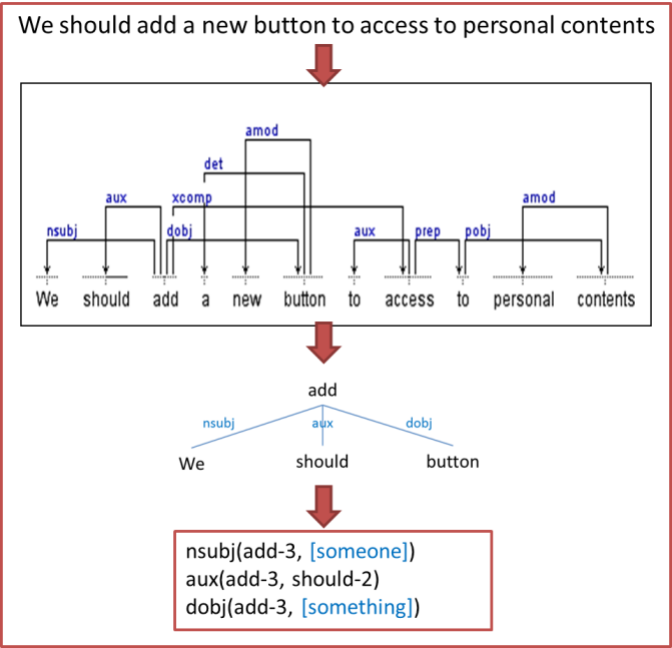
\includegraphics[width=0.40\textwidth]{deca1}
    \bicaption{Q判据等值面图,同时测试一下一个很长的标题,比如这真的是一个很长很长很长很长很长很长很长很长的标题。}{Isocontour of Q criteria, at the same time, this is to test a long title, for instance, this is a really very long very long very long very long very long title.}
    \label{fig:deca1}
\end{figure}

作者通过图\ref{fig:deca1}定义了“【某人】应添加【某事物】”的启发规则并于特征请求相关联。Andrea Di Sorbo等人的观点是在软件工程领域始背相关的重复语言模式,这对软件过程中的需求分析非常有用。

\subsection{基于统计机器学习的需求发现}

\section{聊天对话数据在需求分析中的应用}

\section{自然语言处理中的文本分类}
\subsection{文本嵌入式表达}

\section{少样本学习}


\section{}


